\paragraph{}
Due to the fact that there are a few error indicators, it could be hard to determine the relationship between them and whether a subdomain need refinement or not.
As a result, specific technique is required in order to search for patterns in the data to find this relationship.
After that a final decision which is a binary classification in this case as each subdomain will be labeled as ``refine'' or ``not refine'' can be made based on the input of the error indicators explained before.
Hence, the discovery of regularities plays a key role in adaptive analysis and an automatic discovery of regularities is usually associated with pattern recognition by the help of algorithms.


\paragraph{}
A machine learning algorithm is such an algorithm that is able to learn from data and find regularities.
The ``learning'' is defined as ``A computer program is said to learn from Experience E with respect to some class of tasks T and performance measure P, if its performance at tasks in T, as measured by P, improves with experience E.'' \cite{Mitchell:1997:ML:541177}
The tasks T refer to the task that are too hard to solve with fixed programs.
For example, if a robot is designed to be able to walk, it can be done by a program that help the robot learn how to walk or by a program written manually to tell the robot how to walk.
The second option is rarely chosen because a fixed programs can hardly adapt the complex situation in the reality.
The task in adaptive analysis will be classification.
In this type of task, the algorithm is required to specify which category some input belongs to.
Solving this task is to find a function $f: \mathbb{R}^n \rightarrow \{0,1\}$ where $0$ stands for ``not refine'' and $1$ for ``refine''.
Each variable in the vector of the input $\pmb{x}$ in the function $y=f(\pmb{x})$ is a feature.

\paragraph{}
As a way to measure the abilities of a machine learning program, quantitative measurement of its performance must be designed.
Accuracy could be one of the most popular performance measurement in classification task.
It is simply defined as the rate of examples for which the algorithms gives the same classification as the reality.
In adaptive analysis, the ability that a model performs on data that it has not seen before is more important as it is related to its performance when used in real world problem.
Consequently, these performance measures are usually evaluated using a subset of the original data called test set.
While another subset of the original data called training set are adopted to train the machine learning system.



%   ----    %
\subsection{Training Set}
\paragraph{}
The training set is determined by numerical examples in fig.~\ref{adap_fig:svm_train_chole} and fig.~\ref{adap_fig:svm_train_cantilever}.
The training data is annotated with whether a subdomain is refined or not and the model can study the data and learn to classify each subdomain based on all four features explained in \ref{adap_error_indicator}.
\begin{figure}[!ht]
    \centering
    \begin{subfigure}[b]{0.5\linewidth}
        \scalebox{0.5}{
            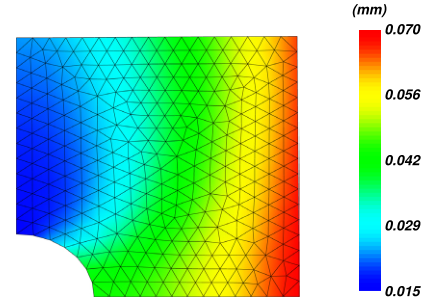
\includegraphics{adaptivity/images/adap_svm_train_chole_0.png}
        }
        \caption{Mesh and displacement field before refinement}
    \end{subfigure}
    \begin{subfigure}[b]{0.5\linewidth}
        \scalebox{0.45}{
            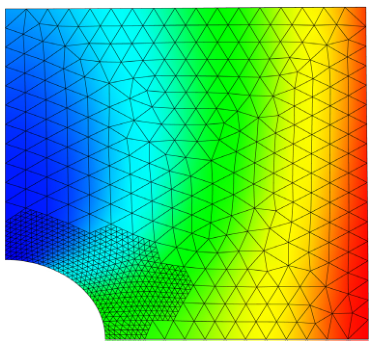
\includegraphics{adaptivity/images/adap_svm_train_chole_1.png}
        }
        \caption{Mesh and displacement field after refinement}
    \end{subfigure}
    \caption{Mesh refinement for square plate with circular hole \cite{Duval2018}}
    \label{adap_fig:svm_train_chole}
\end{figure}

\begin{figure}[!ht]
    \centering
    \begin{subfigure}[b]{0.4\linewidth}
        \scalebox{0.6}{
            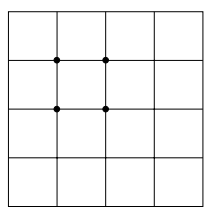
\includegraphics{adaptivity/images/adap_svm_train_cantilever_0.png}
        }
    \end{subfigure}
    \begin{subfigure}[b]{0.4\linewidth}
        \scalebox{0.6}{
            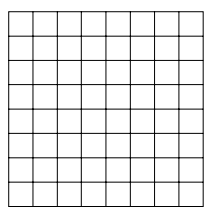
\includegraphics{adaptivity/images/adap_svm_train_cantilever_1.png}
        }
    \end{subfigure}\\
    \begin{subfigure}[b]{1\linewidth}
        \centering
        \scalebox{0.7}{
            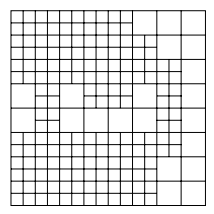
\includegraphics{adaptivity/images/adap_svm_train_cantilever_2.png}
        }
    \end{subfigure}
    \caption{Mesh refinement of a short cantilever beam \cite{Zienkiewicz2005500}}
    \label{adap_fig:svm_train_cantilever}    
\end{figure}

\paragraph{}
With the same examples, uniform mesh of quadtree is conducted and the same region are marked as refined as shown in fig.~\ref{adap_fig:svm_train_my}.
\begin{figure}[!ht]
    \centering
    \begin{subfigure}[b]{1\linewidth}
        \centering
        \scalebox{0.25}{
            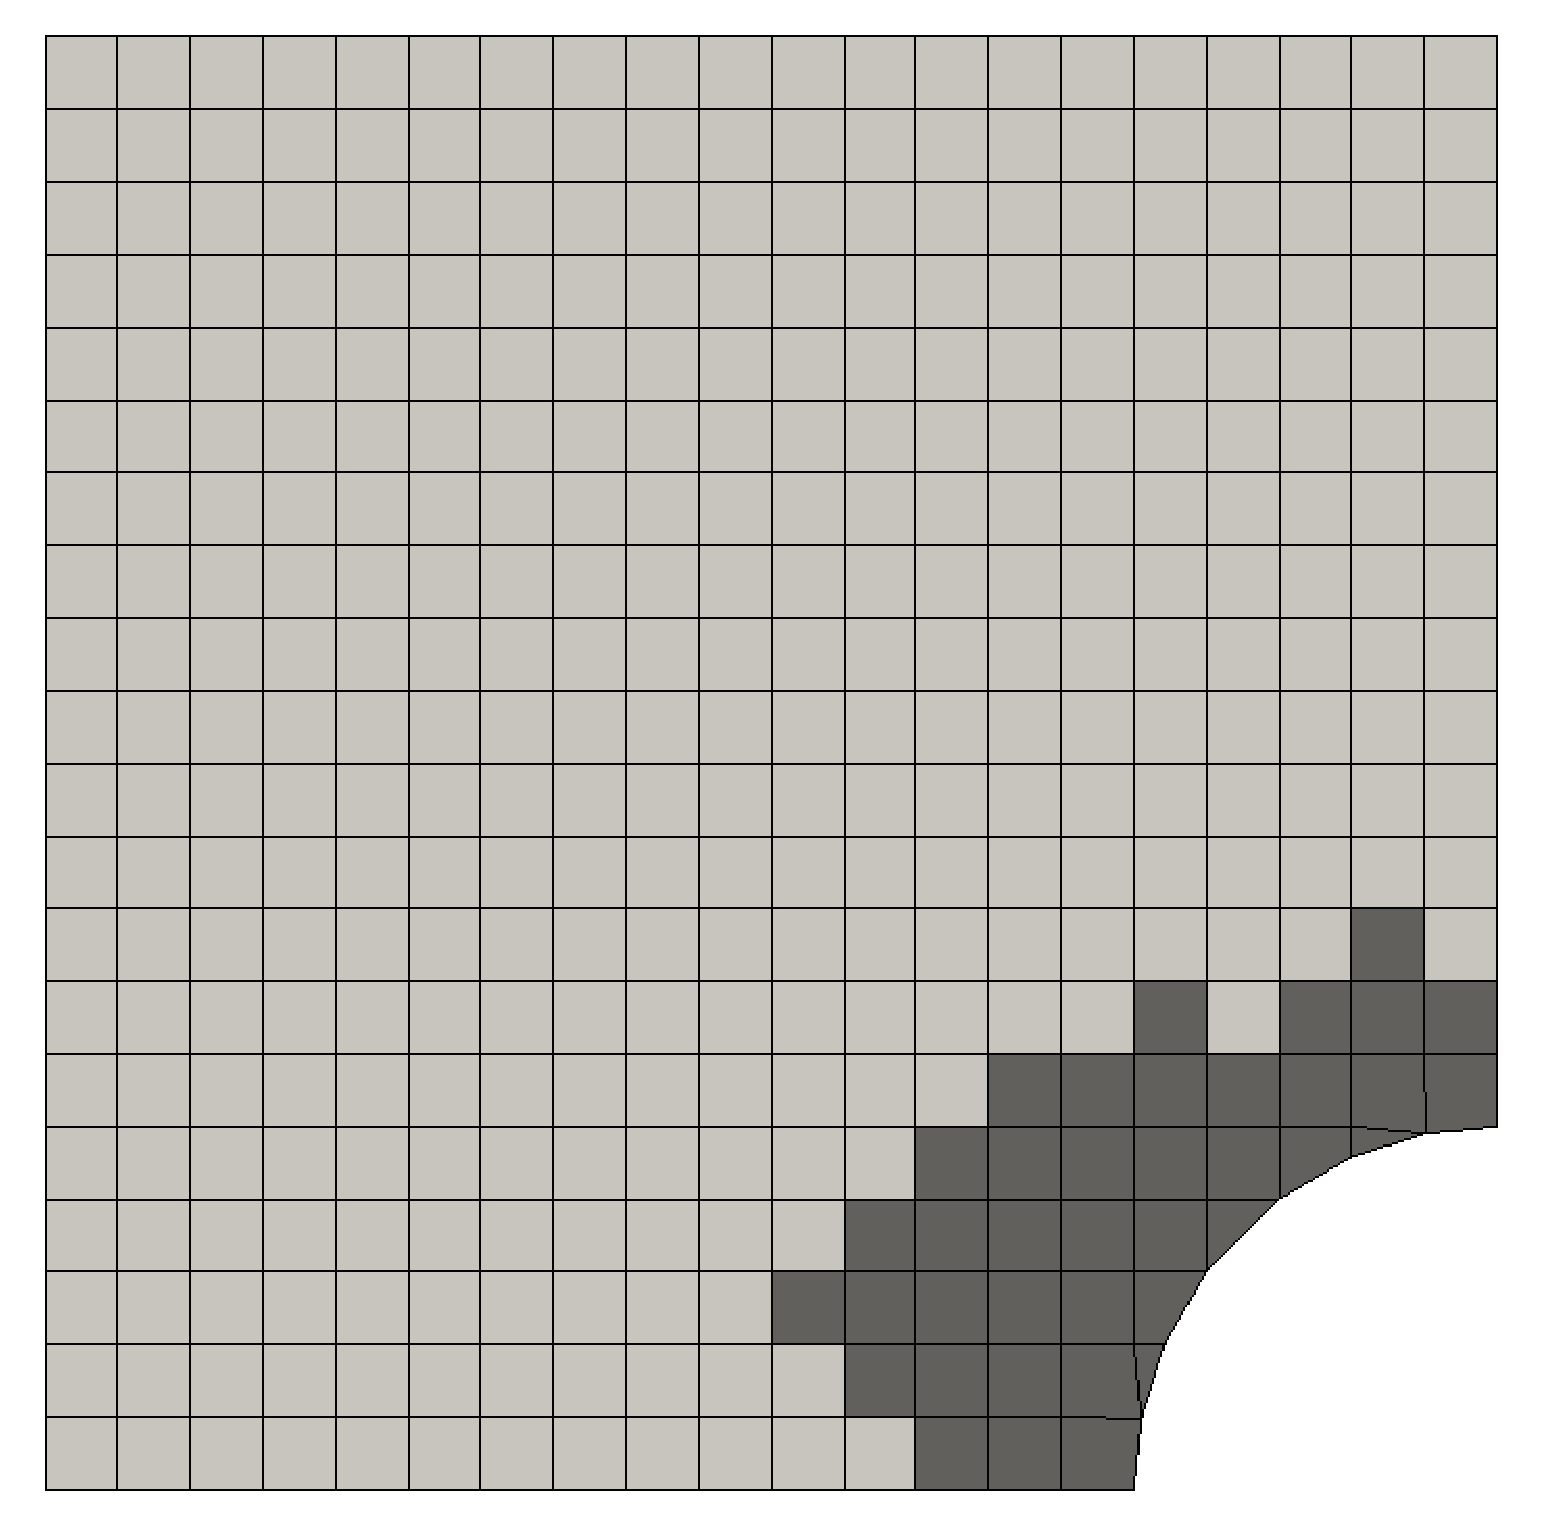
\includegraphics{adaptivity/images/adap_svm_train_my_chole.eps}
        }
    \end{subfigure}
    \begin{subfigure}[b]{0.49\linewidth}
        \scalebox{0.25}{
            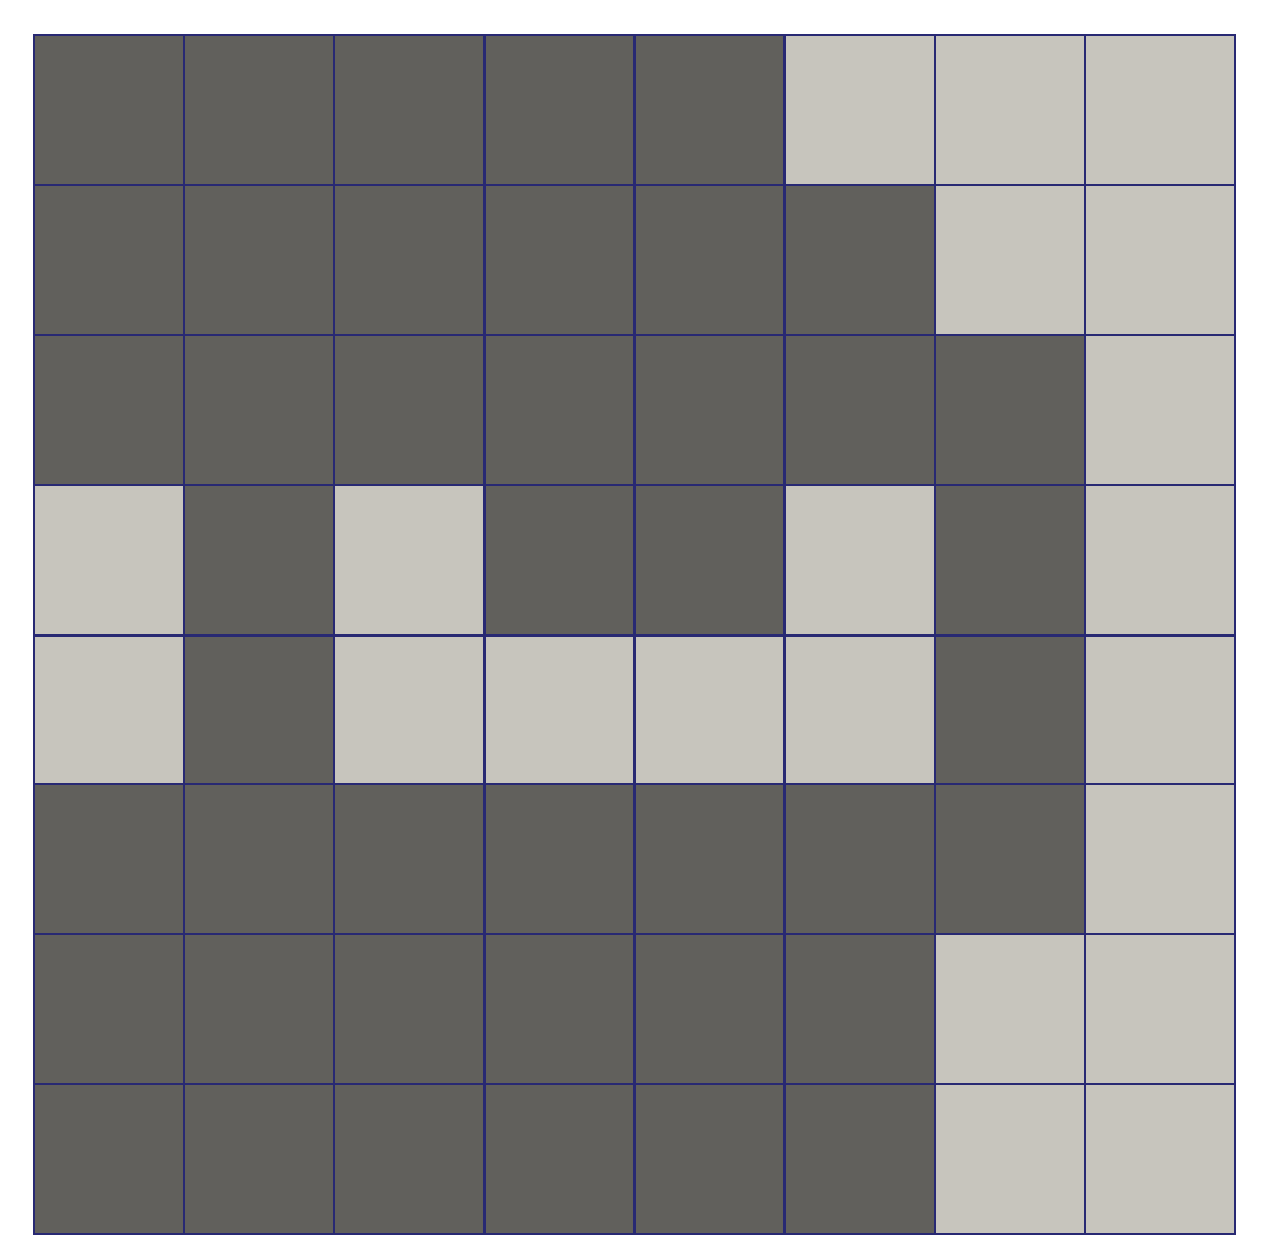
\includegraphics{adaptivity/images/adap_svm_train_my_cantilever_0.eps}
        }
    \end{subfigure}
    \begin{subfigure}[b]{0.49\linewidth}
        \scalebox{0.25}{
            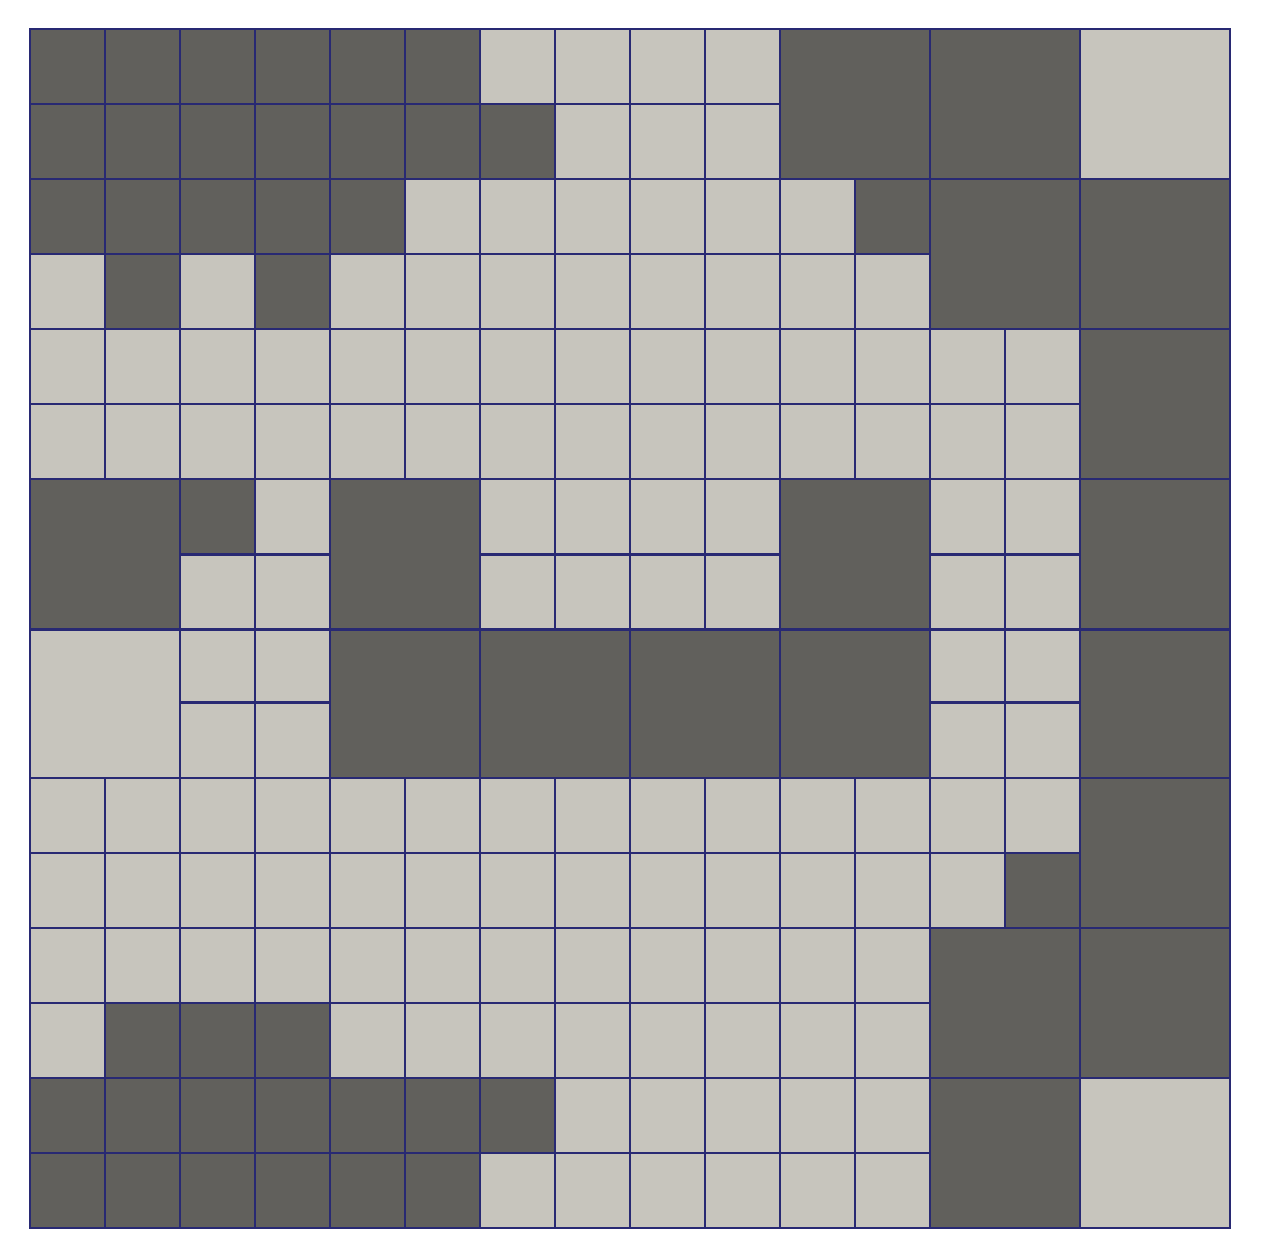
\includegraphics{adaptivity/images/adap_svm_train_my_cantilever_1.eps}
        }
    \end{subfigure}
    \caption[Training data for SVM]{Training data for SVM: Cells in black is marked as refined.}
    \label{adap_fig:svm_train_my}
\end{figure}

Criteria taken into consideration are: 
\begin{enumerate}
    \item Ratio of the area of the cell to the total area
    \item Minimal angle formed by the intersecting lines connected by scaling center and adjacent polygon vertexes
    \item Eigenvalue error indicator for displacement
    \item Eigenvalue error indicator for stress
\end{enumerate}

\subsection{Performance indicators}
\subsubsection{Confusion matrix}
A confusion matrix is a matrix used to illustrate the outcome of a classification model on a set of test data whose actual results are known.
    % Please add the following required packages to your document preamble:
    % \usepackage{multirow}
    \begin{table}[]
        \centering
        \caption{Confusion matrix}
        \label{my-label}
        \begin{tabular}{ccccc}
                                & & \multicolumn{2}{c}{\textbf{Predicted}}                 &  \\ \cline{3-4}
                                \multirow{3}{*}[-0.7em]{\textbf{Actual}} &
                                & \multicolumn{1}{|c|}{Refined}        & \multicolumn{1}{c|}{Not refined}    &  \\ \cline{2-4}        
                                & \multicolumn{1}{|c}{Refined}     & \multicolumn{1}{|c|}{True Positive(TP)}  & \multicolumn{1}{c|}{False Negative(FN)} &  \\ \cline{2-4}
                                & \multicolumn{1}{|c}{Not refined} & \multicolumn{1}{|c|}{False Positive(FP)} & \multicolumn{1}{c|}{True Negative(TN)}  &  \\ \cline{2-4}
        \end{tabular}
    \end{table}
\subsubsection{Accuracy}
\paragraph{}
Accuracy may be the most intuitive indicator.
It is simply defined as $\frac{TP+TN}{TP+TN+FP+FN}$
The importance of accuracy is dependent on the prior since the model can be highly influenced by the prior probability distribution.
For example, a spam detection model is trained from a data set which contains only 10\% of the spam e-mails.
As a consequence, if the model is extremely conservative and classify almost all incoming e-mails as non-spam, it can easily achieve an accuracy of more than90\% in cross validation which is higher than lots of spam detectors.

\subsubsection{Precision(P)}
\paragraph{}
$$P=TP/(TP+FP)$$
Precision describes the chance that the model gives `true' and it is actually `true'.
In the spam detector example, a high precision can be expected as a conservative tends to give non-spam unless it has strong confidence.

\subsubsection{Recall rate(R)}
\paragraph{}
$$R=TP/(TP+FN)$$
Recall rate describes the ratio the model gives `true' to the total number of `true's.
In the spam detector example, a low recall rate is expected.

\subsubsection{F1 score}
\paragraph{}
$$F1 = 2*P*R/(P+R)$$
F1 score is an indicator that consider both the precision rate and the recall rate.
It is defined as the harmonic mean of them.

\subsubsection{Receiver operating characteristic(ROC)}
\paragraph{}
ROC is a True Positive Rate(TPR) vs False Positive Rate(FPR) curve (fig.~\ref{adap_fig:svm_roc}) where $TPR=R$ and $FPR=FP/(FP+TN)$
\begin{figure}[h!]
    \centering
    \scalebox{0.25}{
        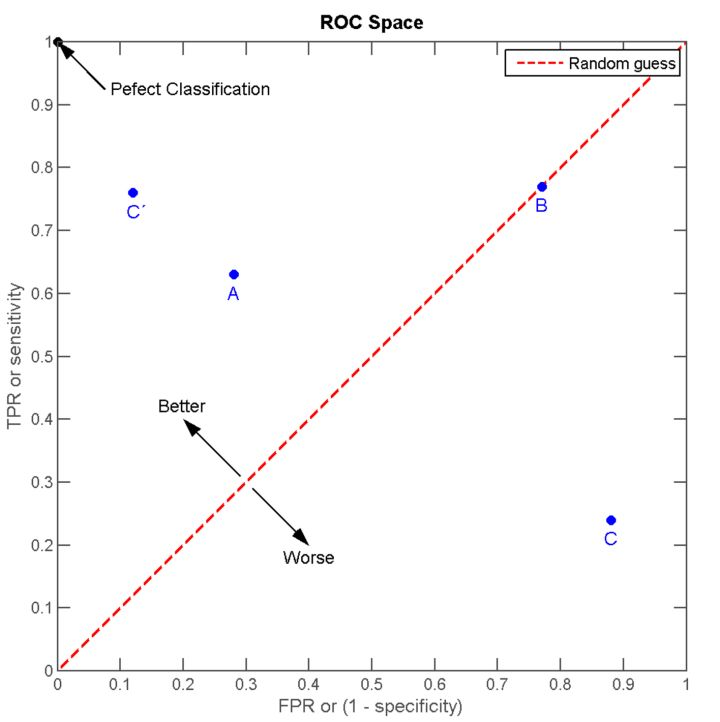
\includegraphics{adaptivity/images/svm_roc.jpg}
    }
    \caption{Receiver operating characteristic(ROC)}
    \label{adap_fig:svm_roc}
\end{figure}

\subsubsection{Area under the curve(AUC)}
\paragraph{}
As can be seen from ROC, the larger the area under the curve, the better the classifier is.
Consequently, area under the curve (AUC) becomes another important indicator in machine learning.

\subsubsection{Indicator used in adaptivity}
\paragraph{}
The balance of the indicators is highly dependent on classifiers' objective.
Take the spam detector for an example, a false positive can be more dangerous than a false negative as an important e-mail being marked as spam can be a disaster.
While in adaptivity, there may be no favour over either of them.
It is because refine a cell with lower error or leave a cell with higher error unrefined may not produce significant influence on the final result.
As a result, F1 score can be the most important indicator as it takes both recall rate and precision into consideration.


\subsection{Result}
\paragraph{}
All training data are standardized by eq.~\ref{adap_eq:svm_standardized} where $\overline{x}$ and $\sigma$ is the mean and standard deviation of the data.
It makes features in training data have zero means and unit variance.
Cell that need to be refined are labeled as $1$ and the rest are labeled as $0$.
Radial basis function with $\sigma=0.7624$ is adopted as kernel function.
    \begin{equation}
        x^\prime = \frac{x-\overline{x}}{\sigma}
        \label{adap_eq:svm_standardized}
    \end{equation}
Half of the training data (320 out of 640) are used to train the model and the reset are used as a cross validation.
Different class weight is set for testing different performance in regard to all indicators in fig.~\ref{adap_fig:svm_performance_0}.
\begin{figure}[h!]
    \centering
    \scalebox{0.3}{
        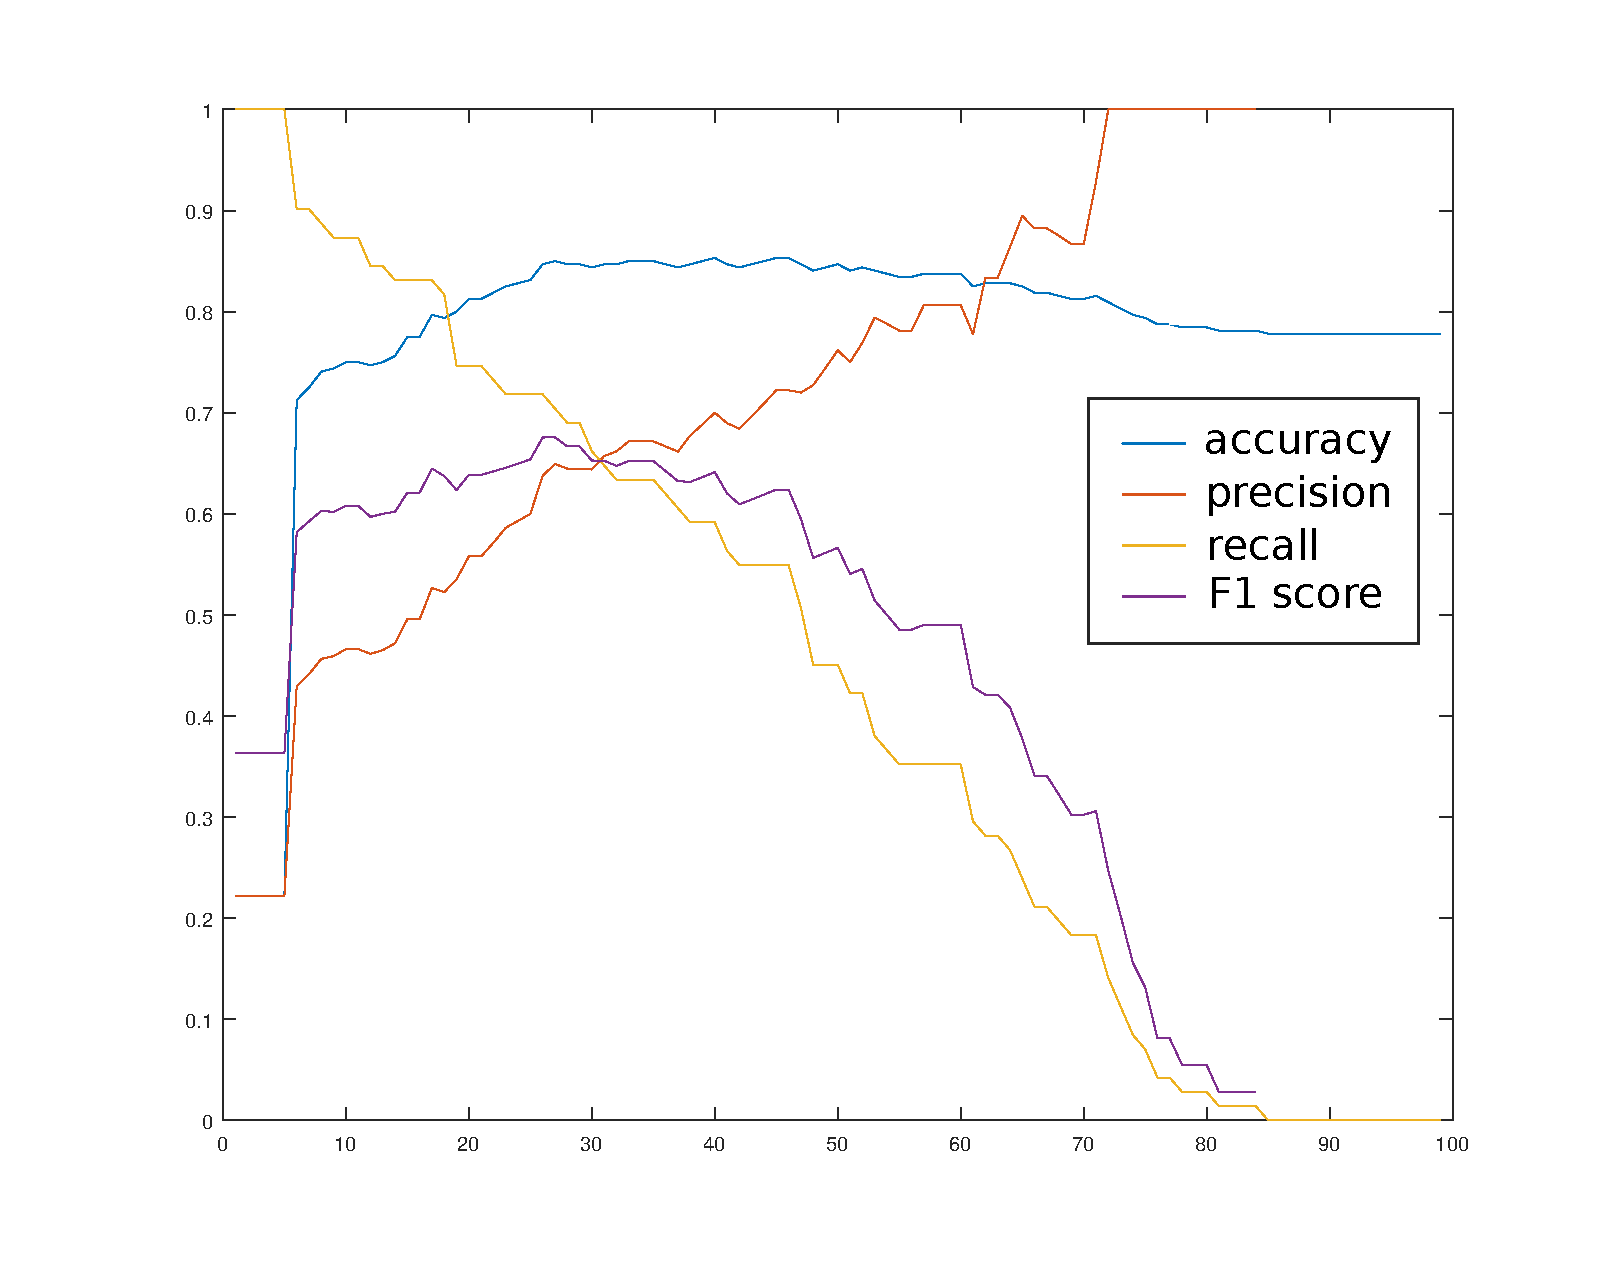
\includegraphics{adaptivity/images/svm_performance_0.eps}
    }
    \caption{Accuracy, precision, recall rate and F1 score vs different class weight}
    \label{adap_fig:svm_performance_0}
\end{figure}
A class weight is a vector that influence the predict directly.
The model will calculate the probability for each classification based on the input and the one with higher probability will be chosen as the result in default situation.
Change class weight to $1:2$ will force the model to choose first class when its probability is more than $66.67\%$ instead of $50\%$.
A class weight of $3:7$ was chosen from fig.~\ref{adap_fig:svm_performance_0} to guarantee a balance between precision and recall rate.
The corresponding result is listed in tab.~\ref{adap_tab:svm_result}.
\begin{table}[h!]
    \centering
    \caption{Result of cross validation}
    \begin{tabular}{cc}
        \toprule
        Accuracy    &   84.38\%    \\
        Precision   &   64.38\%     \\
        Recall rate &   66.20\%     \\
        F1 score    &   65.28\%     \\
        \bottomrule
    \end{tabular}
    \label{adap_tab:svm_result}
\end{table}
%  compare auc
\pagebreak